\section{Scopo e preparazione}

Si intende realizzare un'oscillatore sinusoidale a ponte di Wien con un OpAmp TL081
e osservarne il funzionamento, verificando le relazioni previste con le caratteristiche dei componenti utilizzati.
Si è dunque montato il circuito in \fig{circ}, utilizzato invariato in tutta l'esperienza; i valori misurati
per i componenti sono riportati in \tab{comp_mis}.

\begin{figure}[h]
	\centering
	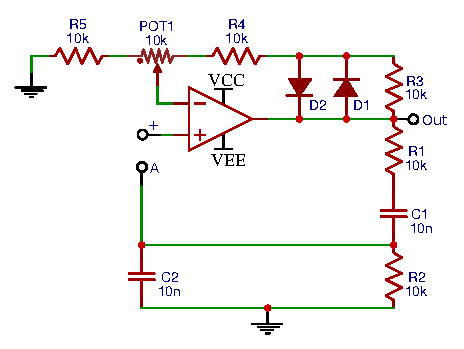
\includegraphics{circuito.pdf}
	\caption{Circuito oscillatore a ponte di Wien.}
	\label{f:circ}
\end{figure}

\begin{table}[h]
	\centering
	\begin{tabular}{ *{5}{S[table-figures-decimal=2]} *{2}{S[table-figures-decimal=1, table-figures-uncertainty=1]} }
		{$R_1$ [\si{\kohm}]} & {$R_2$ [\si{\kohm}]}	& {$R_3$ [\si{\kohm}]} & {$R_4$ [\si{\kohm}]} & {$R_5$ [\si{\kohm}]}
			& {$C_1$ [\si{\nano\farad}]} & {$C_2$ [\si{\nano\farad}]} \\
		\midrule
		9.95(9) & 9.94(9) & 9.90(9) & 9.94(9) & 9.90(9) & 10.8(5) & 10.1(4) \\
	\end{tabular}
	\caption{Misure dei componenti.}
	\label{t:comp_mis}
\end{table}

La sezione superiore del circuito, costituita dai diodi, dal potenziometro e dalle resistenze $R_{3-4-5}$,
è la rete di feedback necessaria ad utilizzare l'OpAmp come amplificatore (non invertente) rispetto all'ingresso non invertente,
mentre la sezione inferiore, costituita dal parallelo e dalla serie di resistenza e condensatore, realizza il feedback di Wien
che, riportato all'ingresso non invertente dell'OpAmp, rende il circuito un oscillatore (a patto che sia verificata la condizione di Barkhausen).

\section{Loop gain}

Intendiamo innanzitutto misuare il guadagno della rete di feedback di Wien: abbiamo dunque collegato l'ingresso
non invertente dell'OpAmp al generatore d'onda e inviato un sengale sinusoidale di ampiezza picco-picco $\approx \SI{500}{\mV}$
a varie frequenze comprese tra \SIrange[range-phrase = \text{ e }]{500}{3000}{\Hz},
misurando il segnale in uscita al punto A del circuito. Utilizzando il softare OpenChoice si sono presi i dati per ogni singola sinusoide in entrata ed uscita. Lo scopo è dunque fare un fit a tali segnali per ottenerne ampiezza,frequenza, fase ed un eventuale offset.Tale procedura è stata eseguita per ogni frequenza nel range prima considerato.
Inseguito si è eseguito un altro fit del guadagno $A=\left | \frac{V_A}{V_+} \right | $ moltiplicato per il termine di feedback $\beta$ in funzione della frequenza secondo la formula $\beta A= (\frac{1}{1+\frac{R_1}{R_2}(1+\frac{\omega_s}{\omega_p}+i(\frac{\omega}{\omega_p}-\frac{\omega_s}{\omega} ))})(1 + \frac{(1-x)Pot+R_4+R_3 \paral D_1 \paral D_2}{R_5+xPot})$. 
\footnote{Si è indicato $\omega=2 \pi f$, $\omega_p= \frac{1}{R_2C_2}$ e $\omega_s=\frac{1}{R_1C_1}$. Si è tenuto conto dei valori reali delle resistenze e dei condensatori che essendo diversi tra loro rendono piu complicata l'espressione di $\beta$. }
Dal fit si sono ottenuti i seguenti valori:\\
$Pot= \SI{}{\kohm}$\\
$x= \SI{}{}$\\ 
$R_diodi= \SI{}{}$\\
$\chi^2 =  ( \dof, p = )$\\
Dal curva di fit inoltre si ricava la frequenza per la quale la fase di $\frac{V_A}{V_+}$ è nulla, che risulta essere ???$\SI{}{\Hz}$.  Dall'analisi del circuito si vede che tale frequenza è $f=\frac{1}{2 \pi \sqrt{R_1C_1R_2C_2}}= \SI{1.53(8)}{\kHz}$.Sono compatibili le due frequenze???

Variando la posizione del potenziometro si osserva che aumentando la resistenza verso $R_5$ si osserva una diminuzione dell'ampiezza del segnale in uscita , viceversa un aumento dell'ampiezza girando dalla parte opposta. Tale comportamento è analogo a quello presente in un OpAmp con feedback solo negativo .
